\subsection{Experimental Setup}

\paragraph{Scenarios}

In this section, we describe the two scenarios that we experiment with,
the historial data we have and choice of parameters of our policy.

The first scenario is based on the real-life case of New York Presbyterian
hospital (NYP). NYP hospital has three different sites for outpatients MRI
across Manhattan. They are named after their address: York Ave, 55th St and
West 84th St. See Figure \ref{fig:site}. The two sites on each side is very
close to each other, it's only 15min walking distance. The one on west side
is a bit further, it's 15min driving distance without traffic.
The patients usually arrive at their site 30min before their appointment
time to prepare so that they can be ready by the appointment time.
Thus, if we call patient 1 hour before their appointment times, this
would mean they have 30min to react to the change. This could be reasonable
given the short distance between the sites. We also experiment with 90min
lead time, which gives patients 60min to react.

\begin{figure}
\centering
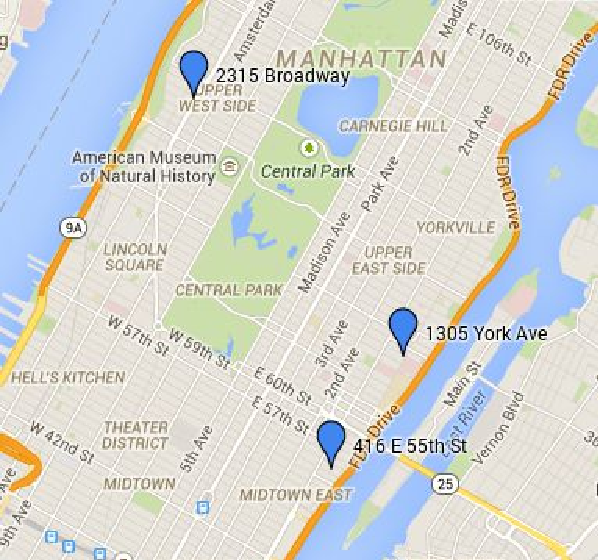
\includegraphics[scale=.6]{chap3/numeric/pic/site.pdf}
\caption{Locations of MRI facilities of New York Presbyterian. There
are three in total represented as blue bubbles. Two of them are on
east side and one is on west side.}
\label{fig:site}
\end{figure}

These sites have different number of MRI machines. West 84th has
only one machine. 55th St has two machines. York Ave has four machines.
Since they have different processing capacity, different number of
appointments are scheduled for. With 4 machines
at York Ave, itself has quite a bit resourcing pooling ability, making
patients there in general wait less.

The second scenario we consider is a system with 7 sites each has one
MRI machine. The reason is that we want to explore the impact of
diversion on a set of small cooperating imaging facilities. Also,
in this case all sites are homogeneous so we can isolate out
the impact of resource pooling without worrying about unbalance in
processing capacities across sites.

\paragraph{Data}
We have three years data of historical MRI scans. For each of these
scans, we have the type of scan, its appointment time, when patient
arrived, when scan began and when scan finished. The data we have
isn't perfect, but we can fit reasonable model inputs from it.

\begin{itemize}
\item Initial schedule for the day. We'd like our schedule to have
  same distribution of scans of each type with the historical one.
  We also know, for each type of scan, the slot size allocated.
  Combining these, we generate synthetic schedules sharing similar
  properties with historical ones.
\item The set of patients who are volunteers. We make the fraction
  of volunteers a parameter that varies across experiments.
  This can help us understand how much impact diversions can have
  given different level of flexbility from patients.
\item Patient arrival time. We fit one empirical distribution on
  the difference between patients' arrival time and appointment time.
\item Preparation time. We don't actually have timestamp data on this.
  We overcome this by looking at the first patients processed each day,
  and use the difference between their arrival time and scan begin time
  as preparation time. Since the first patients don't need to stay in
  waiting room, so it's reasonable to assume all time between arrival
  and scan begin are used for preparation. We fit one empirical distribution
  based on this.
\item Scan duration. For each type of scan, we fit an empirical
  scan duration from historical data.
\item The set of SDAOPs and their arrival time. We get the rate of
  SDAOPs from historical data and generate SDAOPs as Possion process.
\item Cancellations. We calculate the historical probability of cancellation.
  Then for each appointment, we independently make it a cancellation with
  the historical probability.
\end{itemize}
Ideally, we'd like to test our policy by replaying history with real
scan duration, arrival time for each historical appointment. However,
the data we obtain isn't perfect. There are some critical fields missing
so we cannot exactly reconstruct history. Also, there are often
error on timestamps that can greatly impact how the daily schedule looks like.
To prevent these data issues to interfere with our experiments, we choose
to experiment with synthetic schedules.

One can improve the inputs by predicting the scan duration and
arrival time better using more information. For example, the patients'
health condition, diagnosis, home address and other information can be
helpful to make better prediction. However, we don't access to those
sensitive health information.

\paragraph{Parameters}

There are several parameters we need to choose for setting up our simulation
and for our optimization procedure. We describe our choice of them here.

\begin{itemize}
  \item Volunteer probability. We vary the percent of patients who are willing
    to be volunteer. This will allow us to see the effect of our policy
    with varying level of flexibility.
  \item Lead time. We experiment with both 60min and 90min lead time.
  \item Overtime weight $\lambda = 10$, this reflects the fact overtime is quite valuable.
  \item $\theta_c = 0.7, \theta_p = 0.7$. We choose the confidence threshold on objective value
    and waiting time of diverted patient to be neither too aggressive nor too conservative.
  \item The number of samples to evaluate quality of diversions $k=100$.
  \item The number of simulated days to estimate policy performance per experiment $k'=100$.
\end{itemize}
